\documentclass[tikz,border=10pt]{standalone}

\usepackage{xcolor}
\usetikzlibrary{
    arrows.meta,
    positioning,
    fit,
    backgrounds,
    shapes.geometric
}

\begin{document}

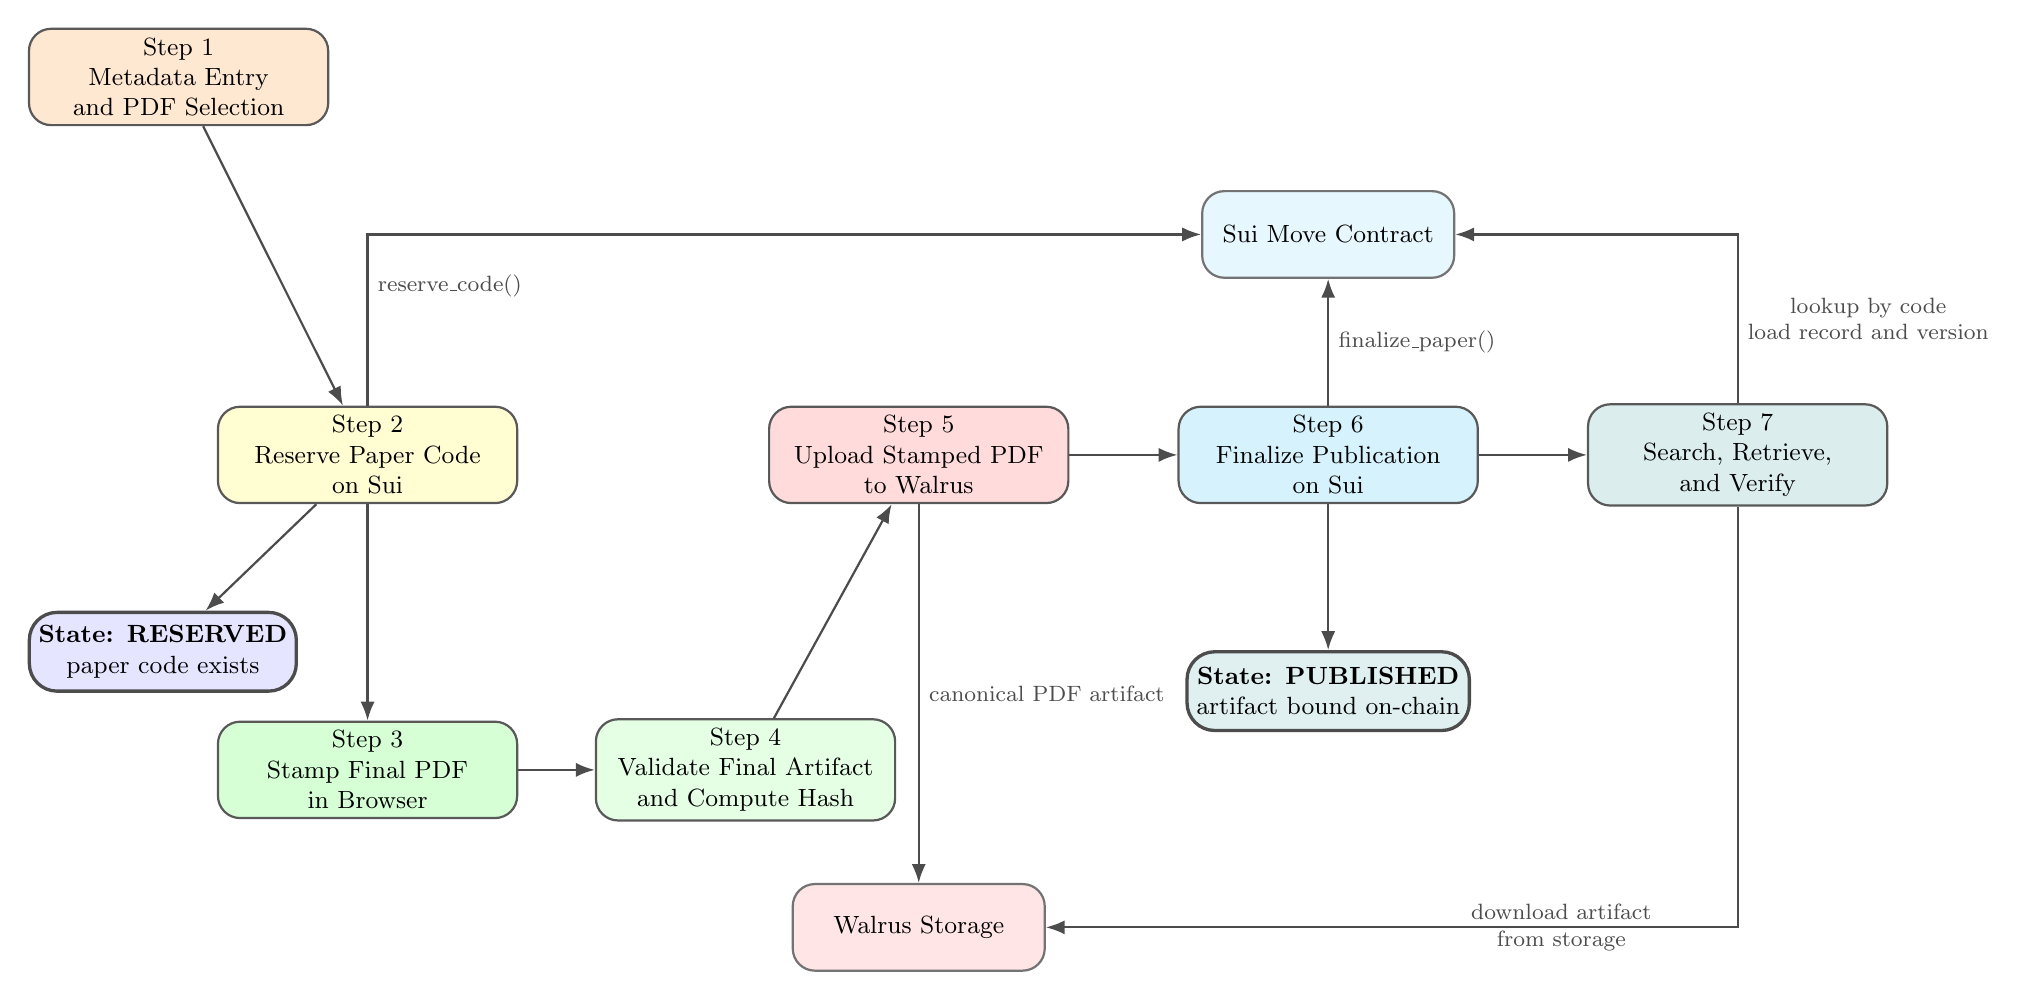
\begin{tikzpicture}[
    font=\small,
    stepbox/.style={
        rectangle,
        rounded corners=8pt,
        draw=black!65,
        thick,
        align=center,
        minimum width=3.8cm,
        minimum height=1.2cm,
        fill=white
    },
    statebox/.style={
        rectangle,
        rounded corners=10pt,
        draw=black!70,
        very thick,
        align=center,
        minimum width=2.9cm,
        minimum height=1.0cm,
        fill=blue!10
    },
    sysbox/.style={
        rectangle,
        rounded corners=8pt,
        draw=black!55,
        thick,
        align=center,
        minimum width=3.2cm,
        minimum height=1.1cm,
        fill=gray!10
    },
    arrow/.style={
        -{Latex[length=2.4mm,width=1.8mm]},
        thick,
        draw=black!70
    },
    note/.style={
        font=\footnotesize,
        align=center,
        text=black!70
    }
]

% =========================================================
% Workflow steps
% =========================================================
\node[stepbox, fill=yellow!18] (step2) at (8.6,0)
{Step 2\\Reserve Paper Code\\on Sui};

\node[stepbox, fill=orange!18] (step1) at (6.2,4.8)
{Step 1\\Metadata Entry\\and PDF Selection};

\node[stepbox, fill=green!16] (step3) at (8.6,-4)
{Step 3\\Stamp Final PDF\\in Browser};

\node[stepbox, fill=green!10] (step4) at (13.4,-4)
{Step 4\\Validate Final Artifact\\and Compute Hash};

\node[stepbox, fill=red!14] (step5) at (15.6,0)
{Step 5\\Upload Stamped PDF\\to Walrus};

\node[stepbox, fill=cyan!16] (step6) at (20.8,0)
{Step 6\\Finalize Publication\\on Sui};

\node[stepbox, fill=teal!14] (step7) at (26.0,0)
{Step 7\\Search, Retrieve,\\and Verify};

% =========================================================
% States
% =========================================================
\node[statebox] (reserved) at (6,-2.5)
{\textbf{State: RESERVED}\\paper code exists};

\node[statebox, fill=teal!12] (published) at (20.8,-3.0)
{\textbf{State: PUBLISHED}\\artifact bound on-chain};

% =========================================================
% Supporting systems
% =========================================================
\node[sysbox, fill=cyan!10] (sui) at (20.8,2.8)
{Sui Move Contract};

\node[sysbox, fill=red!10] (walrus) at (15.6,-6.0)
{Walrus Storage};

% =========================================================
% Main workflow arrows
% =========================================================
\draw[arrow] (step1) -- (step2);
\draw[arrow] (step2) -- (step3);
\draw[arrow] (step3) -- (step4);
\draw[arrow] (step4) -- (step5);
\draw[arrow] (step5) -- (step6);
\draw[arrow] (step6) -- (step7);

% =========================================================
% State transitions
% =========================================================
\draw[arrow] (step2) -- (reserved);
\draw[arrow] (step6) -- (published);

% =========================================================
% System references
% =========================================================
\draw[arrow] (step2) |- node[pos=0.35, right, note] {reserve\_code()} (sui);

\draw[arrow] (step6.north) -- node[midway, right, note] {finalize\_paper()} (sui.south);


\draw[arrow] (step5) -- node[right, note] {canonical PDF artifact} (walrus);

\draw[arrow] (step7) |- node[pos=0.25, right, note] {lookup by code\\load record and version} (sui);
\draw[arrow] (step7) |- node[pos=0.70, right, note] {download artifact\\from storage} (walrus);


\end{tikzpicture}

\end{document}
